% Evans second edition, section 3.5.
% English source: printed p. 154; PDF page 171 (1-based).
% Chinese section starts: checked against the chapter-opening list, PDF p. 79.
% Status: editorial study draft with detailed proofs and mathematical notes; no independent review.
\Needspace{65mm}
\section{Problems}
\label{sec:3-5}

\noindent\textit{Source: Evans \S3.5, Problems 1--20, printed pp.~154--158
(PDF pp.~171--175).} Statements below are concisely restated.
All solutions are editorial, with smoothness assumed where required;
extensions beyond the smooth class are identified explicitly.

\subsection{Problems 1--8: envelopes and characteristics}
\Needspace{30mm}
\paragraph{1. A complete Hamilton--Jacobi integral.}
\begin{proof}[Solution]
For $U=a\cdot x-tH(a)+b$, $D_xU=a$ and $U_t=-H(a)$, proving the PDE.
There are $n+1$ parameters for $n+1$ independent variables.
The derivatives with respect to $a_i$ independently vary $D_xU$;
the derivative with respect to $b$ changes the value by one without
changing any gradient component.
These $n+1$ jet variations are linearly independent, proving completeness.
\end{proof}

\Needspace{30mm}
\paragraph{2. Envelopes of lines and planes.}
\begin{proof}[Solution]
For $G=x_1+a^2x_2-2a$, the stationary condition is $G_a=2ax_2-2=0$.
Thus $a\ne0$, $x_2=1/a$, and $G=0$ then gives $x_1=a$.
The envelope is $x_1x_2=1$, with both branches represented.
The line with $a=0$ has no finite stationary contact.
For $G=2a_1x_1+2a_2x_2-x_3+a_1^2+a_2^2$,
stationarity yields $a_i=-x_i$ and elimination gives
$x_3=-x_1^2-x_2^2$.
The derivatives of this paraboloid equal the slopes $2a_i$ of the
selected plane, directly verifying tangency. The figure in \S3.1
shows both constructions.
\end{proof}

\Needspace{30mm}
\paragraph{3. Eliminate parameters to obtain a PDE.}
\begin{proof}[Solution]
(a) For $\sum_i a_ix_i^2+u^3=0$, implicit differentiation gives
$2a_ix_i+3u^2u_{x_i}=0$.
Multiply by $x_i$, sum, and eliminate $\sum_i a_ix_i^2=-u^3$:
\[
 u^2(3x\cdot Du-2u)=0.
\]
On a nonzero branch this is $3x\cdot Du=2u$.
For a $C^1$ graph it extends to the zero set by continuity from
nonzero points, while on the interior of $\{u=0\}$ the gradient is zero.
This avoids division by a possibly zero coordinate $x_i$.

(b) A unit sphere centered at $(a,0)$ has
$|x-a|^2+u^2=1$. Differentiation yields $x-a=-uDu$.
Substitution eliminates $a$ and gives $u^2(1+|Du|^2)=1$,
on regions where the sphere is a differentiable graph.
\end{proof}
\Needspace{45mm}
\PDEAnnotation{参数消元要记录分支}{除以 $u$、$x_i$ 或某个行列式前，先说明它不为零。得到的简化 PDE 可能丢掉零解或特殊分支；保留未约去的形式有助于检查。}

\Needspace{30mm}
\paragraph{4. Forced transport.}
\begin{proof}[Solution]
For $u_t+b\cdot Du=f(x,t)$, use time as the characteristic parameter:
$\dot X=b$, $\dot Z=f(X,s)$.
Starting from the target, $X(s)=x-(t-s)b$.
Therefore
\[
 u(x,t)=g(x-tb)+\int_0^tf(x-(t-s)b,s)\,ds.
\]
This is the same formula as in Chapter 2.
In the full characteristic system the spatial gradient satisfies
$\dot P=D_xf$ and the time-gradient component satisfies $\dot Q=f_t$.
\end{proof}

\Needspace{30mm}
\paragraph{5. Three characteristic calculations.}
\begin{proof}[Solution]
(a) For $x_1u_{x_1}+x_2u_{x_2}=2u$, start at $(a,1)$.
Then $X=(ae^s,e^s)$, $Z=e^{2s}g(a)$.
For $x_2>0$, $s=\log x_2$ and $a=x_1/x_2$, so
$u=x_2^2g(x_1/x_2)$.

(b) For $x_1u_{x_1}+2x_2u_{x_2}+u_{x_3}=3u$,
start at $(a,b,0)$.
Then $X=(ae^s,be^{2s},s)$, $Z=e^{3s}g(a,b)$, giving
$u(x)=e^{3x_3}g(x_1e^{-x_3},x_2e^{-2x_3})$.

(c) For $uu_{x_1}+u_{x_2}=1$, start at $(a,a)$ with $Z(0)=a/2$.
The equations integrate to
\[
 X_2=a+s,\qquad Z=a/2+s,\qquad X_1=a+(a/2)s+s^2/2.
\]
Eliminate $s=X_2-a$:
$X_1=a(1-X_2/2)+X_2^2/2$.
Thus
\[
 a=\frac{2x_1-x_2^2}{2-x_2},\qquad u(x_1,x_2)=x_2-a/2
\]
locally near boundary points $(a,a)$ with $a\ne2$.
The parameter Jacobian is $1-x_2/2$.
At $(2,2)$ the boundary conditions themselves are incompatible:
Tangential differentiation gives $u_{x_1}+u_{x_2}=1/2$,
whereas the PDE and $u=1$ give the same left side equal to one.
There is no $C^1$ solution through that boundary point.
\end{proof}

\Needspace{30mm}
\paragraph{6. Flow Jacobians and a continuity equation.}
\begin{proof}[Solution]
Let $X(s;x,t)$ solve $\dot X=b(X)$ with $X(t;x,t)=x$.
On any interval where the smooth flow exists, its derivative matrix
$M=D_xX$ satisfies $M_s=Db(X)M$ and $M(t)=I$.
Jacobi's determinant formula gives
\[
 J_s=\operatorname{tr}(M^{-1}Db(X)M)J=(\operatorname{div}b)(X)J,
 \quad J(t)=1.
\]
In particular $J>0$ and is the exponential of the divergence integral.
For the forward map $Y(t;a)$, the desired density satisfies
\[
 \frac d{dt}\big[u(Y(t;a),t)\det D_aY(t;a)\big]=0.
\]
Set the product equal to $g(a)$; differentiating proves
$u_t+b\cdot Du+u\operatorname{div}b=0$.
Inverting the flow then gives
$u(x,t)=g(X(0;x,t))J(0;x,t)$.
A smooth vector field need not have a global complete flow; the formula
is asserted on its actual existence interval unless completeness is assumed.
\end{proof}

\Needspace{30mm}
\Needspace{45mm}
\PDEAnnotation{密度与被搬运的数值不同}{连续性方程保持的是 $u(Y,t)\det D_aY$，因为体积也在变化；纯传输保持 $u(Y,t)$。当速度无散时 Jacobian 为一，两者才在这一点上重合。}
\paragraph{7. A curved noncharacteristic surface.}
\begin{proof}[Solution]
The tangential boundary gradient is fixed. Write admissible gradients
as $D_{\tan}g+\lambda\nu$.
The derivative of their scalar PDE constraint in $\lambda$ is
$F_p\cdot\nu$. Nonvanishing permits local implicit solution for the
normal component. Equivalently, the characteristic column $F_p$ and
the boundary tangent columns form a basis exactly when this scalar
product is nonzero.
\end{proof}

\Needspace{30mm}
\paragraph{8. Verify the implicit conservation formula.}
\begin{proof}[Solution]
Let $a=x-t\mathbf f'(u)$ and $u=g(a)$.
With $D=1+tDg(a)\cdot\mathbf f''(u)\ne0$, differentiate:
\[
 Du=\frac{Dg(a)}D,\qquad
 u_t=-\frac{Dg(a)\cdot\mathbf f'(u)}D.
\]
Hence $u_t+\mathbf f'(u)\cdot Du=0$.
The nonzero denominator is exactly the rank-one determinant from the
characteristic projection. Its loss is not repaired by the implicit
formula itself.
\end{proof}

\subsection{Problems 9--16: variations and convex duality}
\Needspace{30mm}
\paragraph{9. A free initial endpoint.}
\begin{proof}[Solution]
Variations have $V(t)=0$ but arbitrary $V(0)$.
After integration by parts the first variation is
\[
 \int_0^t\left[L_x-\frac d{ds}L_v\right]\cdot V\,ds
                  -L_v(\dot X(0),X(0))\cdot V(0).
\]
First choose $V(0)=0$ to obtain the Euler--Lagrange equation.
Then arbitrary $V(0)$ gives $L_v(\dot X(0),X(0))=0$.
Adding the initial cost $g(X(0))$ adds
$Dg(X(0))\cdot V(0)$, so the new boundary condition is
$L_v(\dot X(0),X(0))=Dg(X(0))$.
\end{proof}
\Needspace{45mm}
\PDEAnnotation{初始代价决定初始动量}{自由起点不代表可以忽略端点项。变分边界项的负号与 $g(X(0))$ 的变化抵消后，得到 $P(0)=Dg(X(0))$，恰好接上 HJ 特征初值。}

\Needspace{30mm}
\paragraph{10. Two Legendre transforms.}
\begin{proof}[Solution]
(a) For $H(p)=|p|^r/r$, $1<r<\infty$, the maximizer of $v\cdot p-H(p)$
is parallel to $v$, with $|p|^{r-1}=|v|$.
Writing $1/r+1/s=1$ gives $L(v)=|v|^s/s$, also valid at $v=0$.
(b) For $H(p)=\tfrac12p^TAp+b\cdot p$, $A$ symmetric positive definite,
stationarity gives $p=A^{-1}(v-b)$.
Substitution gives $L(v)=\tfrac12(v-b)^TA^{-1}(v-b)$.
Positive definiteness makes this stationary point the unique global maximum
of the concave objective.
\end{proof}

\Needspace{30mm}
\paragraph{11. Subdifferential reciprocity.}
\begin{proof}[Solution]
The condition $v\in\partial H(p)$ is
$H(q)\geq H(p)+v\cdot(q-p)$ for every $q$.
It is equivalent to $p$ maximizing $v\cdot q-H(q)$,
hence to $H(p)+L(v)=p\cdot v$.
Using $H=L^*$, the same argument with the roles exchanged is equivalent
to $p\in\partial L(v)$.
For nonsmooth finite convex functions, this uses the supporting-hyperplane
version of the duality established above, rather than an unjustified gradient.
\end{proof}

\Needspace{30mm}
\paragraph{12. A finite-dimensional dual minimum.}
For smooth convex superlinear $L_i$ and $H_i=L_i^*$, prove
\[
 \min_v[L_1(v)+L_2(v)]=\max_p[-H_1(p)-H_2(-p)].
\]
\begin{proof}[Solution]
For any $v,p$, Fenchel's inequalities give
$L_1(v)+L_2(v)\geq-H_1(p)-H_2(-p)$.
The convex superlinear sum has a minimizing $v_*$.
Smoothness gives $DL_1(v_*)+DL_2(v_*)=0$.
Choose $p_*=DL_1(v_*)=-DL_2(v_*)$.
Both Fenchel inequalities are equalities for this pair.
Thus the minimum equals the stated dual maximum, which is attained at $p_*$.
\end{proof}

\Needspace{30mm}
\paragraph{13. A sharper finite-speed radius.}
\begin{proof}[Solution]
Assume here the source's smooth initial datum, with bounded gradient.
At a minimizing $y$ in (HL), differentiation in $y$ gives
$DL((x-y)/t)=Dg(y)$ when $L$ is smooth.
More generally the convex optimality condition is
$Dg(y)\in\partial L((x-y)/t)$.
Reciprocity and differentiability of $H$ give
$(x-y)/t=DH(Dg(y))$.
Thus $|x-y|\leq Rt$ for $R=\sup_y|DH(Dg(y))|$, proving the restricted
minimum formula on the closed ball $\overline B_{Rt}(x)$.
For merely Lipschitz $g$, a minimizing point need not be a differentiability
point of $g$; the coarser coercive radius already proved for (HL)
remains available without that assumption.
\end{proof}

\Needspace{30mm}
\Needspace{45mm}
\PDEAnnotation{不要对不可微的初值硬求导}{Lipschitz 函数几乎处处可微，但指定的最优起点仍可能落在不可微集合。习题 13 的驻点等式使用光滑初值；一般情形可先用不依赖求导的强制性估计。}
\paragraph{14. Distance to a closed set.}
\begin{proof}[Solution]
For $H(p)=|p|^2$, $L(v)=|v|^2/4$.
If the initial cost is zero on a nonempty closed set $E$ and infinity
elsewhere, the extended-value formula reduces to
\[
 \inf_{y\in E}\frac{|x-y|^2}{4t}
              =\frac{\operatorname{dist}(x,E)^2}{4t}.
\]
Closedness and coercivity give a nearest point.
The formula tends to zero on $E$ and to infinity at each point outside
$E$ as $t\downarrow0$. These are extended-value data, outside the
globally Lipschitz-data theorem; this is a computation of the proposed
formula rather than an invocation of that theorem.
For empty $E$, both sides are infinity by convention.
\end{proof}

\Needspace{30mm}
\paragraph{15. Semiconcavity from uniform convexity.}
\begin{proof}[Solution]
The proof in \S\ref{sec:3-semiconcavity} gives all steps:
strong monotonicity of $DH$ makes $DL=(DH)^{-1}$ Lipschitz with
constant $1/\theta$; integrate its increment to obtain the quadratic
upper bound on $L$; add opposite increments; use the same minimizing
starting point and increments $\pm z/t$. The factor is exactly
$1/(\theta t)$.
\end{proof}

\Needspace{30mm}
\paragraph{16. Supremum contraction.}
\begin{proof}[Solution]
Let $\delta=\sup|g_1-g_2|<\infty$.
For every competitor $y$, the objective for $u_1$ is at most that for
$u_2$ plus $\delta$. Taking infima gives $u_1\leq u_2+\delta$.
Interchanging indices gives the reverse bound, so
$\sup|u_1(\cdot,t)-u_2(\cdot,t)|\leq\delta$.
No differentiation or uniqueness theorem is needed.
\end{proof}

\subsection{Problems 17--20: entropy and wave interactions}
\Needspace{30mm}
\paragraph{17. An unbounded Burgers entropy example.}
Consider
\[
 u(x,t)=\begin{cases}
 -\tfrac23(t+\sqrt{3x+t^2}),&4x+t^2>0,\\
 0,&4x+t^2<0.
 \end{cases}
\]
\begin{proof}[Solution]
On the right smooth region write $A=\sqrt{3x+t^2}$.
Then $u_x=-1/A$ and $u_t=-\tfrac23(1+t/A)$,
whereas $uu_x=\tfrac23(1+t/A)$.
Thus Burgers' equation holds there; it also holds in the zero region.
The interface is $\gamma(t)=-t^2/4$.
At that point $A=t/2$, so $u_l=0$, $u_r=-t$.
Its speed $\gamma'=-t/2$ equals $(u_l+u_r)/2$, proving (RH).
The jump is downward and $u_x<0$ on the right.
Hence at every fixed $t>0$, $u$ is nonincreasing and satisfies the
one-sided entropy bound even with constant zero.
The formula has initial trace
$g(x)=0$ for $x<0$ and $g(x)=-2\sqrt{3x}/3$ for $x>0$,
locally in $L^1$.
It is an unbounded entropy example in this local sense, not an element
of the globally bounded uniqueness class stated in \S3.4.3.
\end{proof}
\Needspace{45mm}
\PDEAnnotation{例子与定理的解空间不同}{这题的熵解无界，不能直接套用要求全局 $L^\infty$ 的唯一性定理。验证 PDE、跳跃条件、单边估计后，还需明确它实际属于哪个局部解类。}

\Needspace{30mm}
\paragraph{18. One-sided bounds survive smoothing.}
\begin{proof}[Solution]
If $u(x+h)-u(x)\leq Eh$ for $h>0$, integrate this inequality after
translation against a nonnegative mollifier of mass one:
$u_\varepsilon(x+h)-u_\varepsilon(x)\leq Eh$.
Divide by $h$ and pass to $h\downarrow0$, obtaining
$(u_\varepsilon)'(x)\leq E$.
Only an upper derivative bound is obtained; there is no absolute-value
bound. The same argument in each spatial direction gives the
regularized Hessian bound used in the HJ uniqueness proof.
\end{proof}

\Needspace{30mm}
\paragraph{19. Conservation of mass.}
Assume a continuous integral solution, $f(0)=0$, and a common compact
spatial support on each bounded time interval.
\begin{proof}[Solution]
For a fixed time horizon choose a spatial cutoff equal to one on that
common support and use its product with a time test in (CL).
The flux term is zero: where the spatial cutoff changes, $u=0$
and $f(u)=f(0)=0$.
Thus the distributional time derivative of $\int u(x,t)\,dx$ is zero,
with initial value $\int g$ supplied by (CL).
Continuity of $u$ and the common support make this integral continuous
in time, so the equality holds at every time, not only almost everywhere.
\end{proof}

\Needspace{30mm}
\paragraph{20. Two shocks interacting with one rarefaction.}
For Burgers flux take $g=1$ on $x<-1$, $0$ on $(-1,0)$,
$2$ on $(0,1)$, and $0$ on $x>1$.
\begin{proof}[Solution]
At $-1$, a $1\to0$ shock starts with speed $1/2$:
$\gamma_l=-1+t/2$.
At $0$, a $0\to2$ fan has $u=x/t$ on $0<x<2t$.
At $1$, a $2\to0$ shock starts with speed one:
$\gamma_r=1+t$.

\paragraph{First stage: $0<t<1$.}
The regions from left to right are
\[
 \begin{array}{c|ccccc}
 x&(-\infty,\gamma_l)&(\gamma_l,0)&(0,2t)&(2t,\gamma_r)&(\gamma_r,\infty)\\
 u&1&0&x/t&2&0 .
 \end{array}
\]
The right shock first meets the fan when $1+t=2t$, namely at $t=1$.

\paragraph{Second stage: $1\leq t<2$.}
The right shock now separates $u_l=\gamma_r/t$ from zero, so
$\gamma_r'=\gamma_r/(2t)$.
Matching $\gamma_r(1)=2$ gives $\gamma_r=2\sqrt t$.
The height-two plateau has disappeared.
The remaining regions have $u=1$ for $x<\gamma_l$,
$u=0$ for $\gamma_l<x<0$, $u=x/t$ for $0<x<\gamma_r$,
and zero to the right.
At $t=2$, the left shock reaches the fan's left edge $x=0$.

\paragraph{Third stage: $2\leq t<T$.}
The left shock now separates one from $\gamma_l/t$, hence
$\gamma_l'=(1+\gamma_l/t)/2$.
Multiply by $t^{-1/2}$ to integrate:
$(\gamma_l/\sqrt t)'=1/(2\sqrt t)$.
Matching $\gamma_l(2)=0$ gives
$\gamma_l=t-\sqrt{2t}$.
Between this curve and $\gamma_r=2\sqrt t$, the state is $x/t$;
it is one to the left and zero to the right.
The shocks meet at
\[
 T=(2+\sqrt2)^2=6+4\sqrt2,\qquad X=2\sqrt T=4+2\sqrt2.
\]

\paragraph{Final stage: $t\geq T$.}
Only a $1\to0$ shock remains, of speed $1/2$.
Continuity of its trajectory at the interaction gives
$\gamma(t)=X+(t-T)/2=1+t/2$.
Thus $u=1$ for $x<1+t/2$ and $u=0$ for $x>1+t/2$.
In all stages each smooth piece solves the PDE, each discontinuity
satisfies (RH), and each shock is downward.
The fan has derivative $1/t$ and other smooth pieces have zero derivative;
therefore the global one-sided bound holds. The initial trace and
entropy uniqueness identify this as the required solution.
Values assigned exactly on the shock curves do not change the weak solution.
\Needspace{45mm}
\PDEAnnotation{最终激波位置可用质量再检查}{相对于 $x=0$ 处的 $1\to0$ 阶跃，初值的积分差为 $-1+2=1$。最终阶跃应比速度 $1/2$ 的参考激波右移一，故为 $x=t/2+1$。}
\end{proof}
\Needspace{45mm}
\PDEAnnotation{进入稀疏波后速度会变}{激波两侧的值不再是两个固定常数，而包含 $\gamma(t)/t$，所以速度要重新由 Rankine--Hugoniot 求出。不能把初始的两条直线一直延长到所有时间。}
\begin{center}
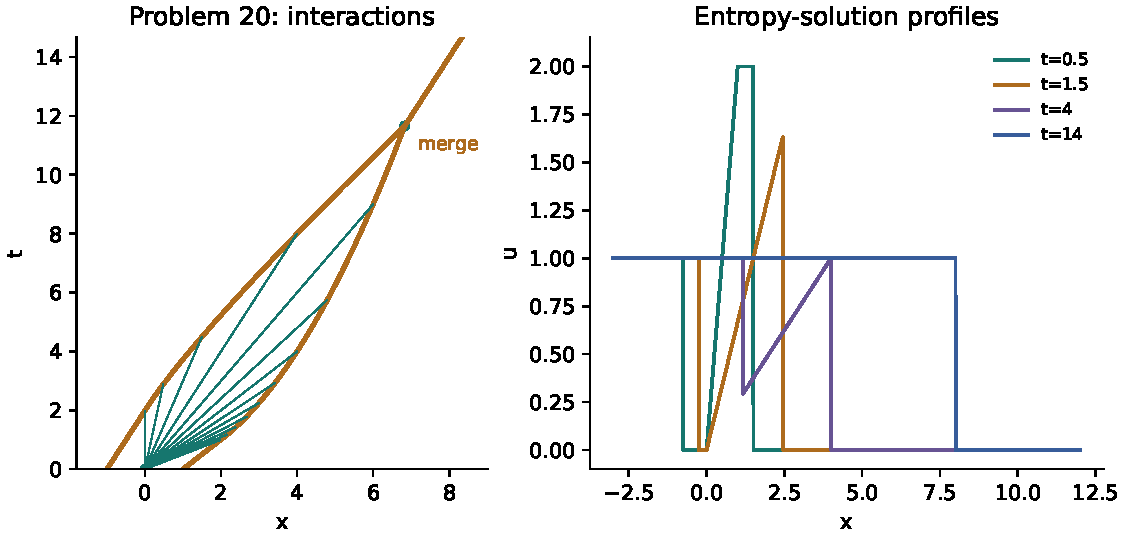
\includegraphics[width=\linewidth]{output/figures/ch03-interacting-waves.pdf}
\end{center}
\noindent\textit{Editorial figure.}
The space-time plot records interactions at $t=1$, $t=2$ and $T$;
the profiles show all four stages. Independent piecewise Hopf--Lax
minimization checks the formulas numerically away from shock ties.
